\documentclass[10pt]{article}

\usepackage{amsmath, amssymb, amsthm}
\usepackage{graphicx}
\usepackage[shortlabels]{enumitem}
\usepackage{xcolor}
\usepackage{listings}
\usepackage{charter}
\usepackage{geometry}
\usepackage{fancyhdr}
\usepackage{algpseudocode}
\usepackage{url}
\usepackage{algorithm}
\usepackage{float}
\usepackage{natbib}
\bibliographystyle{plain}


\geometry{
    letterpaper,
    top=1in,
    bottom=1in,
    left=1in,
    right=1in,
    headheight=15pt,
    headsep=0.25in
}


\pagestyle{fancy}
\fancyhf{}
\renewcommand{\headrulewidth}{0.4pt}
\lhead{\textbf{COMP3106 Final project}}
\cfoot{\thepage}


\newcommand{\eps}{\epsilon}
\renewcommand{\implies}{\rightarrow}
\newcommand{\xor}{\oplus}
\newcommand{\same}{\leftrightarrow}


\theoremstyle{definition}
\newtheorem{theorem}{Theorem}[section]
\newtheorem{lemma}[theorem]{Lemma}
\newtheorem{corollary}[theorem]{Corollary}
\newtheorem{definition}[theorem]{Definition}
\newtheorem{example}[theorem]{Example}

\DeclareMathOperator*{\argmax}{arg\,max}
\DeclareMathOperator*{\argmin}{arg\,min}

\begin{document}

\begin{titlepage}
    \begin{center}
        \vspace*{1cm}
        \textbf{Achieving Optimal Blackjack Play Through Double Q-Learning}\\
        \textbf{COMP3106 Final Project}\\
        \textbf{Qayam Damji (101287631)}\\
        \textbf{Shri Vaibhav Mahesh Kumar(101287156)}\\
        \textbf{Daniel Tam(101267869)}\\
        \vspace{0.8cm}
        Carleton University\\
        Prof.\ Holden\\
        \today
    \end{center}
\end{titlepage}

\tableofcontents
\newpage

\section{Statement of Contribution}
Each of us made an approximately equal contribution to the project. 
\begin{itemize}
    \item Qayam researched and implemented the core of the learning process for the agent, created the demo application and wrote the technical portion of the report.
    \item Daniel implemented the environment and state representation used by the agent, as well as writing the discussion and results section of the report.
    \item Shri implemented the code that performs statistical analysis of model strategy, as well as generating the plots used in the report. He also made the largest contribution to the proposal, and wrote the intro to the paper.
\end{itemize}
\section{Introduction}

\subsection{Background and Motivation}
Blackjack represents an intriguing intersection of skill and chance, making it an ideal environment for exploring reinforcement learning techniques. This project was motivated by the challenge of developing an intelligent agent capable of making optimal decisions in a  probabilistic game environment. The inherent complexity of Blackjack—with its nuanced rules, strategic decision-making, and element of randomness—provides a compelling test for advanced machine learning algorithms.
The fun of this project lies in its potential to create an AI system that can learn and adapt to the intricate strategies of a casino game. Unlike deterministic environments, Blackjack requires balancing risk, probability, and strategic thinking, which makes it an excellent domain for testing and refining intelligent decision-making algorithms.

\subsection{Related Prior Work}
Some prior work that relates to our selected model, algorithm, and task is Q Learning, Double Q learning, and poker research conducted by FAIR(Facebook AI Research). Q Learning was a reinforcement learning technique introduced by Christoper Watkins. It allowed for agents to learn optimal action-value functions through iterative experience. This was based on estimating the value of state-action pairs and determining the best move. This was then further developed by Hado van Hasselt in 2010 to introduce double Q learning. By introducing two separate Q Value estimates, the algorithm mitigates the overestimation bias found in traditional Q learning algorithms. This was very important in stochastic environments, such as our current environment of Blackjack, since overly optimistic value estimates can affect the decision making. FAIRS poker research also helped in pioneering applying reinforcement learning to strategic games.Their work on Poker demonstrated the potential of AI in information-imperfect games. In 2017, FAIR and CMU researches helped develop an AI that was able to defeat professional poker players, showcasing how these advances reinforcement leaning technique can navigate complex, probabilistic and stochastic environments, such as Blackjack.
\subsection{Statement of Objectives}
Develop a Q-Learning agent capable of playing Blackjack at a optimal level, integrating advanced techniques like Double Q-Learning.
Implement a comprehensive learning environment that captures the nuanced rules and strategic complexity of Blackjack, including features like card counting and multiple action spaces.
Systematically optimize the agent's performance through rigorous hyperparameter tuning and validation against standard Blackjack strategies.
Analyze the learned strategy to understand how the agent develops decision-making patterns that approach or potentially exceed traditional basic Blackjack strategy.

\section{A Formal Definition of Blackjack}
Blackjack is the most widely played casino game in the world, due to it's intoxicating combination of skill and chance.
The fact that it is incredibly simple to play, (but hard to master), quick, and very social make it a staple in casinos worldwide.

Blackjack is played between individual players and a dealer, with each player having their own independent game against the house. 
The game begins with players placing their bets, after which the dealer deals two cards to each player and themselves. 
Players' cards are typically dealt face-up, while the dealer takes one card face-up (known as the "upcard") and one face-down (the "hole card").

The goal is to beat the dealer by building a hand that totals closer to 21 than the dealer's hand, without exceeding 21. 
Cards 2 through 10 are worth their face value, while face cards (Jacks, Queens, and Kings) are worth 10. 
Aces possess flexibility, being worth either 1 or 11, depending on which value benefits the hand more. 
A hand containing an Ace counting as 11 is called a "soft" hand, as its total can drop by 10 (by converting the Ace to a 1) without busting.

After receiving their initial two cards, players must decide how to play their hand. 
They can "hit" to request additional cards, or "stand" to keep their current total. 
Players may continue hitting until they either decide to stand or their total exceeds 21, resulting in a "bust" and immediate loss of their bet. 
"splitting" permits players to divide a pair of matching cards into two separate hands, each requiring an additional bet equal to the original wager.

The dealer plays their hand last, following strict rules that eliminate any decision-making. 
The dealer must hit on any total of 16 or below and stand on any total of 17 or above (though some casinos require dealers to hit on a "soft 17").
If the dealer busts, all remaining players win. 
If the dealer does not bust, each player's hand is compared to the dealer's, with the higher total winning. 
Equal totals result in a "push," and the player's bet is returned.

\subsection{Basic Blackjack Strategy}
\begin{itemize}
    \item Always hit on hard totals of 8 or below, and stand on hard totals of 17 and above.
    \item Hit on soft totals of 17 or below, and stand on soft totals of 19 or above. 
    \item For hard totals of 12-16, stand if the dealer's upcard is 6 or lower (except hit 12 against 2 or 3), and hit if the dealer shows 7 or higher.
    \item For pairs, always split aces and 8s, never split 5s or 10s, split 2s and 3s against dealer's 4-7, and split 6s against dealer's 2-6.
    \item (SOURCE)
\end{itemize}
\subsection{How to Get Kicked Out of a Casino}
In order to gain an edge, skilled Blackjack players employ techniques classified under the umbrella term "card counting".
There are many different techniques for card counting, varying in complexity and effectiveness.
The general idea is to track which cards remain in the deck being dealt from, in order to make educated predictions on when to hit or stand.
Our agent is provided with the information for Hi-lo card counting during training:
\begin{itemize}
    \item Hi-lo card counting assigns values to cards seen during play: 
    \item low cards (2-6) are worth 1
    \item mid-range cards (7-9) are 0
    \item high cards (10s through Aces) are -1
\end{itemize}
The player keeps a running count of these values as cards are dealt. When divided by the number of remaining decks, 
this gives a "true count." A positive count suggests many high-value cards remain, increasing the chances of strong hands and blackjacks, 
so players should bet more. A negative count indicates many low cards remain, favoring the dealer, so players should minimize bets. (SOURCE)

\section{Methodology}
\subsection{The Environment}
The state space $S$ is represented as a 6-tuple:
\[(player\_value, has\_usable\_ace, dealer\_upcard, count\_bucket, is\_pair, pair\_value)\]

Each component provides information for decision-making:

\begin{enumerate}
    \item \textbf{player\_value} ($\in [4,21]$): The current total value of the player's hand. 
    \item \textbf{has\_usable\_ace} ($\in \{0,1\}$): Indicates whether the player has an Ace that can be counted as 11 without causing a bust. 
    \item \textbf{dealer\_upcard} ($\in [1,10]$): The visible card of the dealer's hand.
    \item \textbf{count\_bucket} ($\in \{-1,0,1\}$): Represents the true count of the deck using the Hi-Lo card counting system, bucketed into three categories:
    \begin{itemize}
        \item -1: Negative count (deck rich in low cards)
        \item 0: Neutral count
        \item 1: Positive count (deck rich in high cards)
    \end{itemize}
    \item \textbf{is\_pair} ($\in \{0,1\}$): Indicates whether the player's initial two cards are a pair, enabling split decisions.
    \item \textbf{pair\_value} ($\in [0,10]$): The value of each card in the pair if is\_pair is true, 0 otherwise. This allows for specific pair-based strategies.
\end{enumerate}
The action space $A$ consists of three possible actions:

\(A = \{0 \text{ (Stand)}, 1 \text{ (Hit)}, 2 \text{ (Split)}\}\)

Each action has specific conditions:

\begin{enumerate}
    \item \textbf{Stand (0)}: The player keeps their current hand and ends their turn. Always available.

    \item \textbf{Hit (1)}: The player draws one additional card. Available unless the hand has busted.

    \item \textbf{Split (2)}: Available only when:
    \begin{itemize}
        \item The hand contains exactly two cards of equal value
        \item The hand hasn't already been split (tracked by split\_depth)
        \item The maximum number of splits (3) hasn't been reached
    \end{itemize}
    When executed, creates two separate hands, each receiving one additional card.
\end{enumerate}

The environment implements several realistic constraints:

\begin{enumerate}
    \item \textbf{Maximum Splits}: Limited to 3 splits per round to prevent infinite splitting
    \item \textbf{Dealer Rules}: Dealer must hit on soft 17 or below, stand on hard 17 or above
    \item \textbf{Natural Blackjack}: Special payouts (1.5x) for natural blackjacks (21 with first two cards)
\end{enumerate}
\subsection{Q-Learning}
We have employed Q-Learning \cite{watkins1992qlearning}, a model-free reinforcement learning algorithm that learns a state-action value function \(Q(s,a)\)
representing the predicted cumulative future reward of taking action \(a\) in state \(s\). 
The values of \(Q(s,a)\) are generated through experimentation in the environment and updated through the following equation:
\[Q(s,a)\leftarrow Q(s,a)+\alpha[r(s)+\gamma\max_{a^\prime}Q(s^\prime,a^\prime)-Q(s,a)]\]
Where:
\begin{itemize}
    \item $\alpha$ is the learning rate
    \item $\gamma$ is the discount factor
    \item $R$ is the immediate reward
    \item $s'$ is the next state
    \item $\max_{a'} Q(s',a')$ is the maximum expected future reward
\end{itemize}
We make use of a dynamic learning rate: 
\[\alpha(s,a) = \max(\alpha_0 \cdot \delta^{N(s,a)}, \alpha_{\min})\]
where \(N(s,a)\) is the visit count and \(\delta\) is the decay rate.

\subsection{Double Q-Learning}
The Double Q-Learning Technique \cite{hasselt2010double} is employed here, 
as it has been shown to reduce overestimation bias in highly stochastic environments, like blackjack.
This technique encorporates two Q-Tables (\(Q_1,Q_2\)) and the following update function:
\[Q_1(s,a) \leftarrow Q_1(s,a) + \alpha[R + \gamma Q_2(s',\arg\max_{a'} Q_1(s',a')) - Q_1(s,a)]\]
\subsection{Warm Start \& the Reward Function}
The reward function we have created is nuanced, going beyond simple binary win/loss based rewards in order to encourage optimal play.
The reward function is designed in order to teach behavior like encouraging safe play when at risk of busting, and hitting on lower totals to reach stronger hands.
\begin{equation}
    R(p,d) = \begin{cases}
    -1.2b & \text{if } p > 21 \\
    1.1b & \text{if } d > 21 \\
    1.5b & \text{if } p = 21 \text{ (natural)} \\
    1.1b & \text{if } p > d \text{ and } p \geq 20 \\
    b & \text{if } p > d \\
    -b & \text{if } p < d \\
    0 & \text{if } p = d
    \end{cases}
\end{equation}
Where \(p=\)the value of the player's hand, and \(d=\)the value of the dealer's hand.\\
\subsection{Epsilon-Greedy Exploration}
The implementation uses an adaptive epsilon-greedy strategy for action selection. \cite{tokic2011adaptive}
The probability of selecting action $a$ in state $s$ is given by:
\begin{equation}
    P(a|s) = \begin{cases}
    1-\epsilon + \frac{\epsilon}{|A|} & \text{if } a = \arg\max_{a'} Q(s,a') \\
    \frac{\epsilon}{|A|} & \text{otherwise}
    \end{cases}
\end{equation}
The exploration rate $\epsilon$ follows a performance-based decay mechanism:
\begin{equation}
    \epsilon = \max(\epsilon_{\min}, \epsilon \cdot \begin{cases}
    \delta_\epsilon \cdot 1.1 & \text{if improving} \\
    \delta_\epsilon & \text{otherwise}
    \end{cases})
\end{equation}
Where:
\begin{itemize}
    \item $\epsilon_{\min}$ is the minimum exploration rate
    \item $\delta_\epsilon$ is the base decay rate
    \item "Improving" is determined by comparing recent average rewards to best seen
\end{itemize}

\subsection{Prioritized Experience Replay}
We use prioritized experience replay to focus learning on the most informative transitions.\cite{schaul2016prioritized}
Transitions are sampled with probability:
\begin{equation}
    P(i) = \frac{p_i^\alpha}{\sum_k p_k^\alpha}
\end{equation}

The priority $p_i$ is the priority based on temporal-difference error:

\begin{equation}
    p_i = |\delta_i| + \epsilon
\end{equation}

Where:
\begin{itemize}
    \item $\delta_i$ is the TD-error: $\delta_i = r + \gamma \max_{a'} Q(s',a') - Q(s,a)$
    \item $\epsilon$ is a small constant ensuring non-zero probability
    \item $\alpha$ determines the strength of prioritization
\end{itemize}
\subsection{Hyperparameter Optimization Implementation}

The Q-learning agent's hyperparameters are optimized through a systematic grid search framework. 
The optimization process explores the parameter space $\Theta$ through scikit-learn's ParameterGrid \cite{scikit_parametergrid}:

\[
\Theta = \{\theta_1 \times \theta_2 \times \cdots \times \theta_n\}
\]
The system employs parallel processing to efficiently evaluate configurations.\\
The optimal configuration $\theta^*$ is selected based on win rate maximization:

\[
\theta^* = \argmax_{\theta \in \Theta} m_{\text{win}}(\theta)
\]
\subsection{Training Algorithm}
\begin{algorithm}[H]
\caption{Double Q-Learning with Prioritized Replay \& Epsilon-Greedy Exploration}
\begin{algorithmic}[1]
\State Initialize replay buffer $\mathcal{D}$
\For{episode = 1 to N}
    \State Initialize state $s$
    \While{not terminal}
        \State Select action $a$ using epsilon-greedy
        \State Execute $a$, observe $r$, $s'$
        \State Store transition $(s,a,r,s')$ in $\mathcal{D}$
        \If{time to update}
            \State Sample batch from $\mathcal{D}$ using priorities
            \State Update either $Q_1$ or $Q_2$ randomly
            \State Update transition priorities
        \EndIf
        \State $s \gets s'$
    \EndWhile
    \State Update $\epsilon$ based on performance
\EndFor
\end{algorithmic}
\end{algorithm}
\subsection{Validation}
The validation of the Q-learning agent's performance was conducted as follows:
\subsubsection{Training Validation}
During the training phase, several metrics were continuously monitored and logged:
\begin{itemize}
    \item Win rate ($\frac{\text{wins} + 0.5 \cdot \text{draws}}{\text{total games}} \cdot 100\%$)
    \item Average reward per game
    \item Split rate ($\frac{\text{splits}}{\text{total games}} \cdot 100\%$)
    \item Blackjack rate ($\frac{\text{blackjacks}}{\text{total games}} \cdot 100\%$)
    \item Bust rate ($\frac{\text{busts}}{\text{total games}} \cdot 100\%$)
\end{itemize}
\subsubsection{Strategy Analysis}
The learned strategy was analyzed through three distinct matrices:
\begin{enumerate}
    \item Hard totals: Player values (12-21) vs. Dealer up-card (2-11)
    \item Soft totals: Player values with usable ace vs. Dealer up-card
    \item Pairs: Split decisions for each possible pair vs. Dealer up-card
\end{enumerate}
These matrices were compared against basic strategy to validate the agent's learning of optimal play patterns.
\section{Results}
\subsection{The Search for Optimal Hyperparameters}
We trained close to 700 different models over 50,000 episodes, yielding the following hyperparameter configuration as "best":
\begin{itemize}
    \item \(\alpha=0.001\)
    \item Batch Size=64
    \item Buffer Size=50000
    \item \(\epsilon=0.05\)
    \item \(\epsilon\) decay=0.99995
    \item \(\min\epsilon=0.01\)
    \item \(\gamma=0.97\)
    \item Learning Rate Decay: 0.9999
\end{itemize}
\subsection{Training Metrics}
Our final agent was trained over 500,000 episodes, resulting in the following:
\begin{itemize}
    \item Win rate: 48.05\% 
    \item Average reward per game: -0.003
    \item Split rate: 3.05\%
    \item Blackjack rate: 5.3\%
    \item Bust rate: 10.95\%
\end{itemize}

\begin{figure}[H]
    \centering
    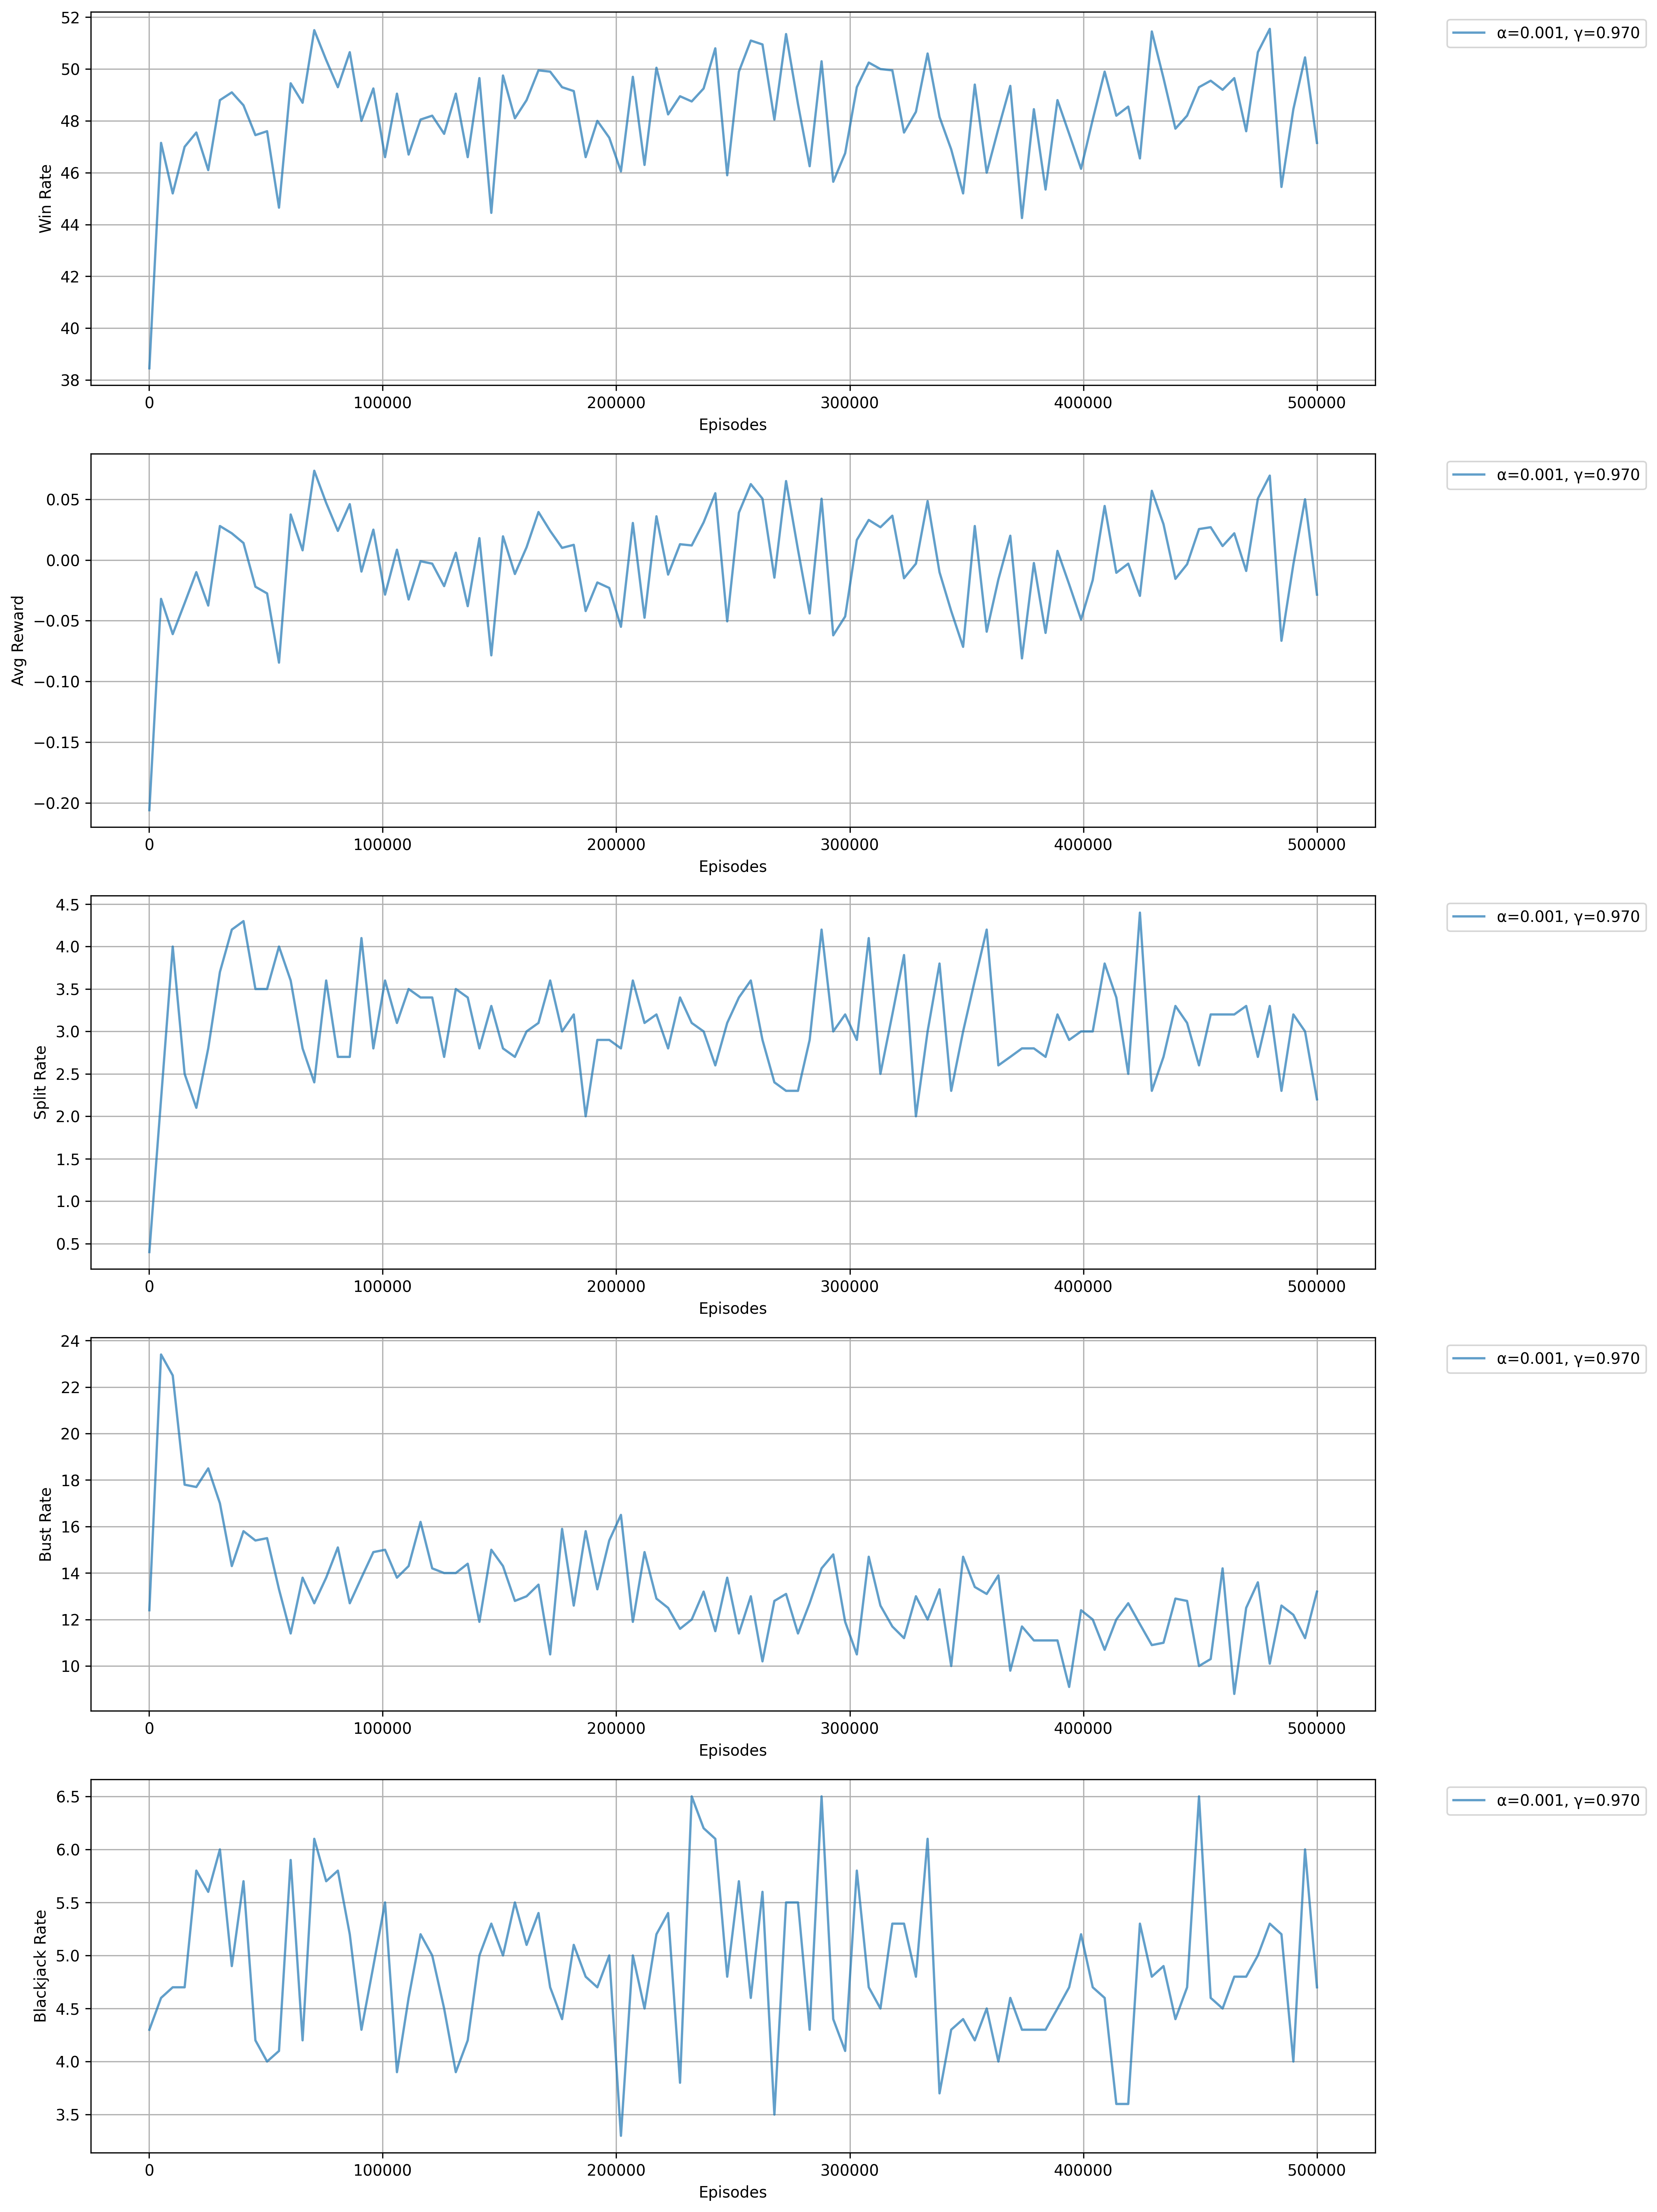
\includegraphics[width=\textwidth]{./images/learning_curves_summary.png}
    \label{fig:training_metrics}
\end{figure}
Upon analysis of the training metrics (Figure \ref{fig:training_metrics}), we came to the following conclusions:
\begin{enumerate}
    \item \textbf{Win Rate Stability}: The win rate stabilized around 48-50\%, showing consistent performance against the house edge. This approaches the theoretical maximum for perfect basic strategy play.

    \item \textbf{Average Reward Convergence}: The average reward per episode converged near zero (-0.003), indicating the agent learned to minimize losses effectively. The low reward variance (1.060491) suggests consistent play rather than high-risk strategies. Consistency is expected of Q-Learning!

    \item \textbf{Strategic Behavior Evolution}:
    \begin{itemize}
        \item The split rate settled around 3\%, suggesting that splitting could have been "taught" more effectively.
        \item The bust rate showed a drastic improvement from initial rates, moving from $>20\%$ to a final rate of 10.95\%
        \item The blackjack rate sat around 5.3\%, which is to be expected with theoretical probability
    \end{itemize}
\end{enumerate}
\subsection{Reviewing the Learned Strategy}

Analysis of the final strategy matrices (Figure \ref{fig:strategy_matrices}) revealed decision-making patterns that mostly align with basic blackjack strategy.

\begin{figure}[H]
    \centering
    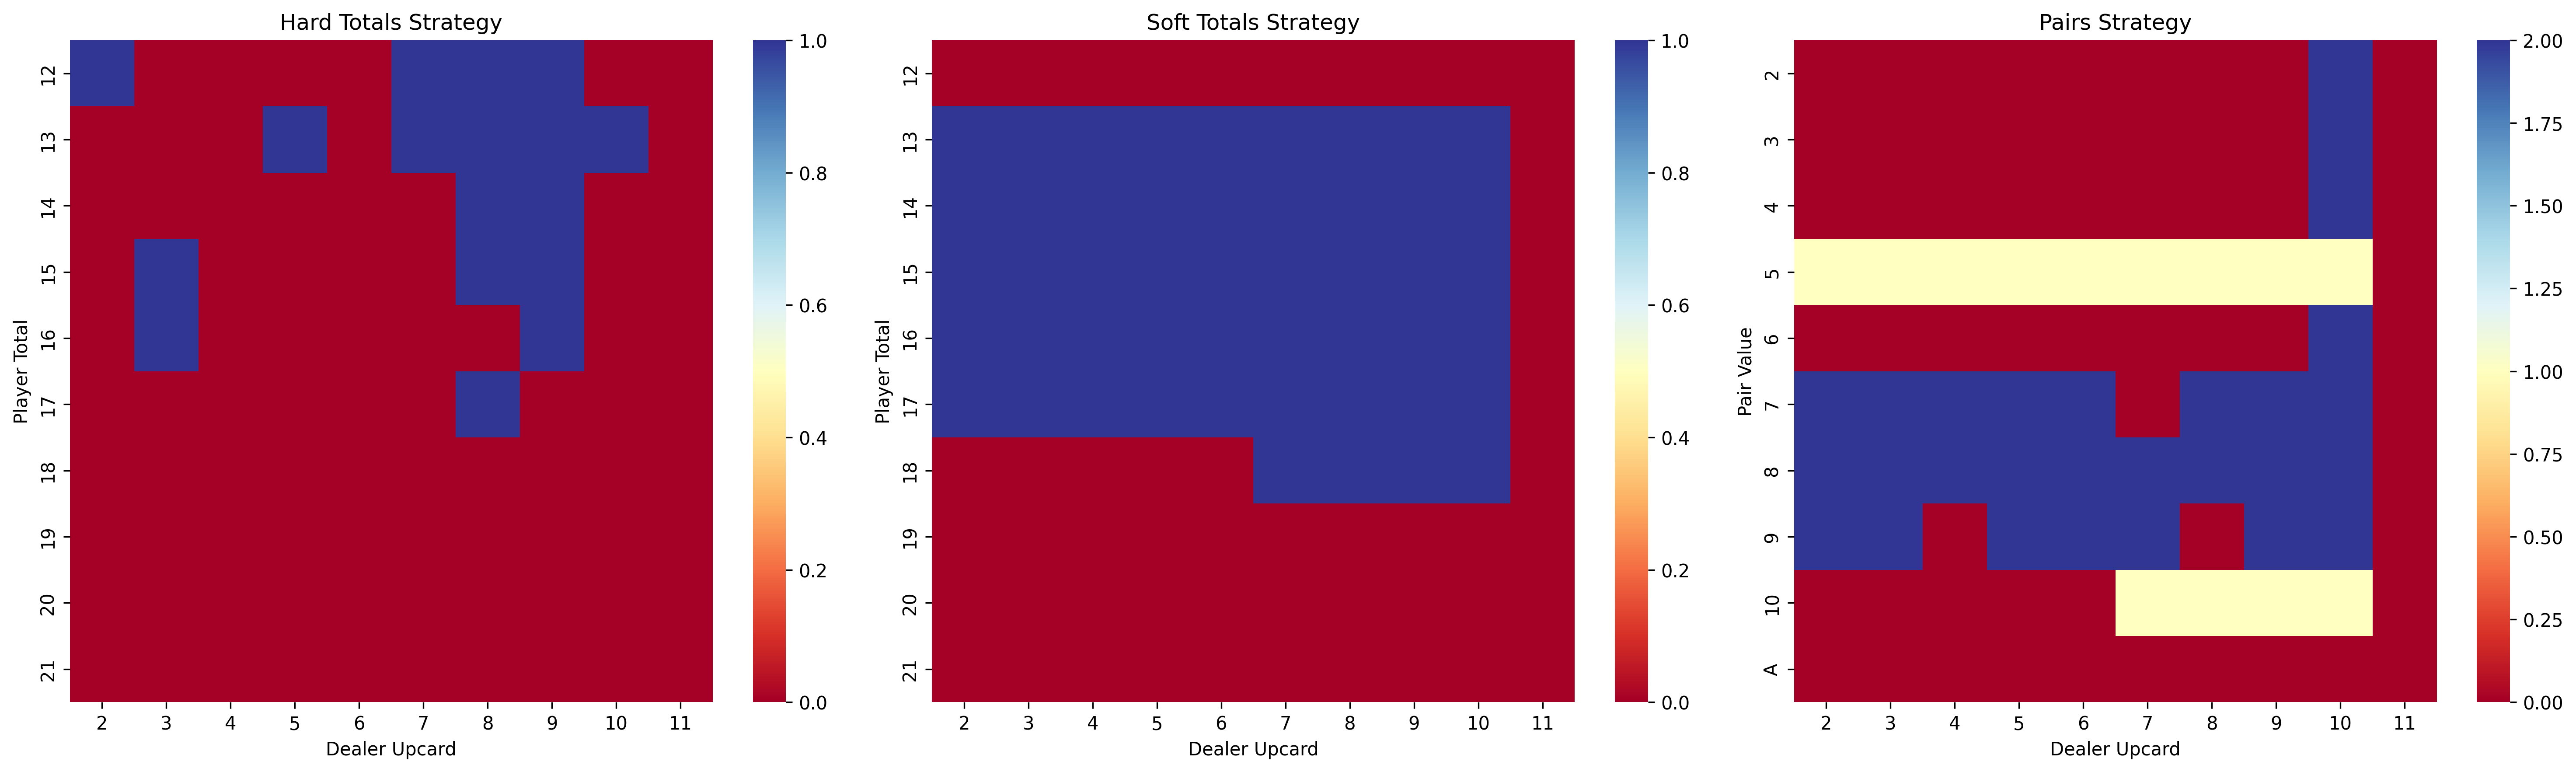
\includegraphics[width=\textwidth]{./images/agent_strategy.png}
    \caption{Final learned strategy matrices}
    \label{fig:strategy_matrices}
\end{figure}

\subsubsection{Hard Totals Strategy}
The hard totals matrix shows clear decision boundaries that follow conventional wisdom:
\begin{itemize}
    \item Stand (red) dominates for player totals 17 and above
    \item Hit (blue) is preferred for most totals 16 and below against high dealer cards
    \item Safe play is adopted against dealer's 2-6, particularly with player totals 13-16
\end{itemize}

\subsubsection{Soft Totals Strategy}
The soft totals matrix demonstrates clever handling of ace-containing hands:
\begin{itemize}
    \item Aggressive hitting on soft totals below 18
    \item Standing on soft 19 and above
    \item Strategic hitting on soft 18 against dealer's strong cards (9-A)
    \item The pattern suggests the agent learned to effectively make use of the flexible nature of aces
\end{itemize}

\subsubsection{Pairs Strategy}
The pairs matrix reveals selective splitting behavior that again, is close to optimal strategy:
\begin{itemize}
    \item Always split aces and eights (blue regions)
    \item Never split fives and tens (red regions)
\end{itemize}
The combination of nearly optimal win rate, low bust rate, show that the agent has learned to balance risk and reward effectively while incorporating card counting information to make better decisions than basic blackjack strategy allows.
\section{Discussion}
\subsection{Limitations}
\subsubsection{Performance Ceiling}
Despite using advanced techniques like Double Q-Learning, Prioritized Experience Replay, and adaptive epsilon-greedy exploration, 
the agent's win rate plateaued/stabilized around 48-50\%. 
This suggests inherent challenges in completely overcoming the house edge in Blackjack. 
This limiation makes sense with real world experience since Blackjack is inherrently desgined with a built in house advantage, 
making it challenging to achieve a state where the agernt can beat the casino.The agent does however approach the theoritical maximum for strategic play.
\subsubsection{Splitting Strategy}
The low split rate (3.05\%) indicates that the agent did not fully learn the nuanced strategies for splitting pairs. 
Future work could focus on more explicitly teaching and incentivizing strategic splitting behaviors such as refining 
the reward function or training. The current reward structure might not inventizite splitting the pairs as a strageic 
option and instead shows as a high risk low reward action. Maybe modifying the reward function to inventivize splitting 
when neccessary can hepl increate the split rate and maybe even increase the win rate the agent has.
\subsubsection{Casino Simulation Fidelity}
The research environment, while comprehensive, may not perfectly replicate real-world casino conditions. 
Variations in dealer rules, deck composition, and other subtle factors could impact strategy transferability. 
We could have inputs to allow the model to train under various dealer rules, to help better accustom it to real world 
experience and hence find the best strategy that works over multitudes of dealer rules as well as deck compisition to 
even the mechanism used to shuffle a deck.
\subsection{Implications}
The research offers several significant implications for reinforcement learning and game strategy:
Advanced Learning in Stochastic Environments: This work demonstrates the potential of combining techniques like Double Q-Learning, 
Prioritized Experience Replay, and adaptive exploration to effectively learn strategies in complex, probabilistic environments such as card games. 
This work showcases how these techniques work together and where they shine vs where they could use some improvement.
\subsubsection{Strategic Learning Beyond Basic Rules}
The agent's ability to approximate and sometimes exceed basic Blackjack strategy highlights the power of machine learning to 
discover nuanced decision-making patterns through iterative learning. 
The agent can pick the right actions to maximize winning chances based on its previous experience showcases that even 
though the game is in the House's Favor, strategic play can get close to 50
\% win rate using the nuanced techniques.
\subsubsection{Card Counting Integration}
By incorporating the Hi-Lo card counting system into the state representation, 
the research showcases how additional contextual information can enhance machine 
learning performance in strategic games.By having the state space enriched with the bucket count of {-1,0,1},
the agent was able to expand trhe tradiantional state representation and acces more contexual information to help 
decide on which actions to take.This additional dimensiality helps transforms the state space from a simple game 
state description to a more dynamic appraoch.
\bibliography{references}
\end{document}